\documentclass[12pt]{article}

% Any percent sign marks a comment to the end of the line

% Every latex document starts with a documentclass declaration like this
% The option dvips allows for graphics, 12pt is the font size, and article
%   is the style

\usepackage[pdftex]{graphicx}
\usepackage{amsfonts}
\usepackage{amsmath}
\DeclareMathOperator*{\max_bottom}{max}
\usepackage{url}
\usepackage{hyperref}

\usepackage{caption}
\usepackage{subcaption}


\hypersetup{
    colorlinks=true,
    linkcolor=blue,
    filecolor=magenta,      
    urlcolor=cyan,
    pdftitle={Sharelatex Example},
    bookmarks=true,
    pdfpagemode=FullScreen,
}


\usepackage{graphicx}
\graphicspath{ {./images/} }

% These are additional packages for "pdflatex", graphics, and to include
% hyperlinks inside a document.

\setlength{\oddsidemargin}{0.5cm}
\setlength{\evensidemargin}{0.5cm}
\setlength{\topmargin}{-1.6cm}
\setlength{\leftmargin}{0.5cm}
\setlength{\rightmargin}{0.5cm}
\setlength{\textheight}{24.00cm} 
\setlength{\textwidth}{15.00cm}
\parindent 0pt
\parskip 5pt
\pagestyle{plain}

% These force using more of the margins that is the default style
\newcommand{\namelistlabel}[1]{\mbox{#1}\hfil}
\newenvironment{namelist}[1]{%1
\begin{list}{}
    {
        \let\makelabel\namelistlabel
        \settowidth{\labelwidth}{#1}
        \setlength{\leftmargin}{1.1\labelwidth}
    }
  }{%1
\end{list}}


\begin{document}
\title{\Large Introduction to machine learning - Homework 3}

\author{
  \textbf{Uri Kirstein}\\
  777777777 \\ aaaaa@campus.technion.ac.il
  \\ \\
  \textbf{Pavel Rastopchin}\\
  321082026 \\ pavelr@campus.technion.ac.il
  \\ \\ 
}

\maketitle


\begin{abstract}
Abstract...
\end{abstract}

\newpage
\section{Process and significant decisions}
In this paragraph we will describe the process of our work.
\subsection{Automatic model selection}
As a part of non-mandatory assignment, we will implement the automatic model selection as an integral part of the mandatory assignment. For such task, we encapsulated all model evaluation scripts in one class called $modelSelector()$ (in short - Selector). As we have 3 prediction tasks, the Selector will train all candidate models on training set, and test all of them on the validation set. The difference between the tasks is that different performance metrics will be used. At the end of validation, each model will get a score for it's performance for each prediction task.

\subsection{Different models for different tasks}
As it stated in the assignment document -  "one size doesn't fit all", i.e. different models can be the best models for each task. To handle this, we decided to include in our $modelSelector()$ class an option to select best model for each task. At the time of writing this paragraph we still don't know if the same model will be selected for all tasks or not.

\subsection{No one-hot representation of Categorical data}
During the work on this submission, we noticed a negative effect of one-hot representation of categorical data on all models performance. Thus we have decided not to convert the categorical data to one-hot representation.


\newpage
\section{Candidate models}
In this section we discuss the candidate models which were selected for our experiments. For the task of most probable voters, we need to predict probabilities, but not the exact tag, so we want to use models which can provide this functionality. Based on post in \href{https://www.researchgate.net/post/What_are_the_best_supervised_classifiers_to_classify_the_problem_of_multiclass_classification}{www.researchgate.net} stating that SVM, KNN and Random Forest can successfully handle a problem of multi-class classification, we decided to choose those two models in addition to a MLP, resulting a total of four candidate models.

\subsection{Hyper parameters tuning with k-fold cross validation}
In order to select the best model candidates, we need to perform 3-fold cross validation using training set only. The cross validation process for all models implemented in $crossValidator$ class. In all our cross-validation experiments we used the $accuracy$ as model performance measurement. Although its not the same measurement we selected for each task, it's still more strict requirement than all other metric we will describe in next sections.

\begin{figure}[h]
\centering
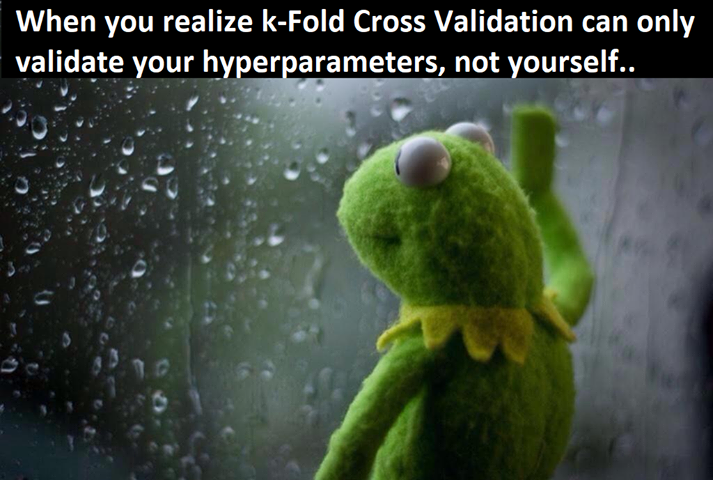
\includegraphics[width=0.5\textwidth]{report_pics/frog}
\caption{A sad fact about hyper-parameters tuning}
\end{figure}

\newpage
\subsection{Support vector machine}
Support vector machines are a set of supervised learning methods used for classification, regression and outliers detection. Main advantages of support vector machines are: Effective in high dimensional spaces, Still effective in cases where number of dimensions is greater than the number of samples. Based on a post in  \href{https://www.researchgate.net/post/Is_it_necessary_to_choose_kernels_in_SVM_according_to_application}{www.researchgate.net} the most important parameters for SVM are the kernel and the C parameter. While the kernel determines the shape of separating hyperplane, the C parameter responsible for overfitting capabilities of the model. A larger C makes the model more complex and lowers its bias, hence it have higher chance of overfitting. A low C gives a model with low variance and high bias. As we could not achieve convergence with linear kernel, we will use SVM with RBF kernel.

\begin{figure}[h]
\centering
\begin{subfigure}{.4\textwidth}
  \centering
  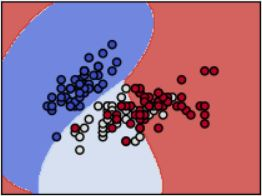
\includegraphics[width=.7\linewidth]{report_pics/SVM_RBF}
  \caption{RBF kernel}
  \label{fig:sub1}
\end{subfigure}%
\begin{subfigure}{.4\textwidth}
  \centering
  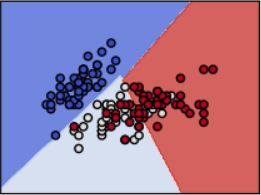
\includegraphics[width=.7\linewidth]{report_pics/SVM_linear}
  \caption{Linear kernel}
  \label{fig:sub2}
\end{subfigure}
\caption{SVM kernel types}
\label{fig:test}
\end{figure}

To select the right value for C hyper parameter we used the k-fold cross validation technique. First we performed cross-validation of a big range of C values with exponential steps and got a plot. Then we repeated the process with smaller range and smaller steps for fine tuning. As we can see from the plots, the best accuracy achieved with C = 20 after which we can't see any improvement, thus this value with be selected for SVM model.

\begin{figure}[h]
\centering
\begin{subfigure}{.5\textwidth}
  \centering
  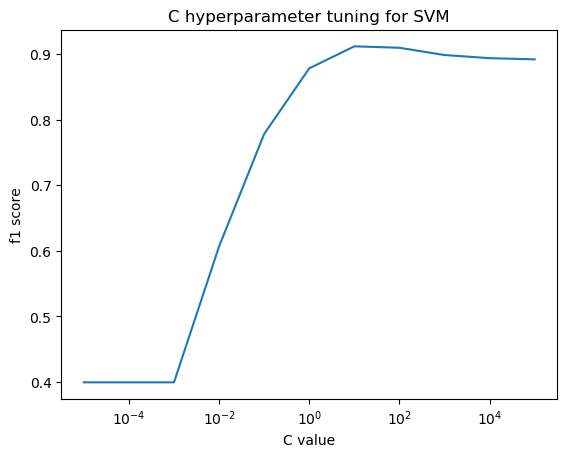
\includegraphics[width=.6\linewidth]{Cross_valid_plots/SVM_C_hyper_fig_coarse.png}
  \caption{C coarse tuning}
  \label{fig:sub1}
\end{subfigure}%
\begin{subfigure}{.5\textwidth}
  \centering
  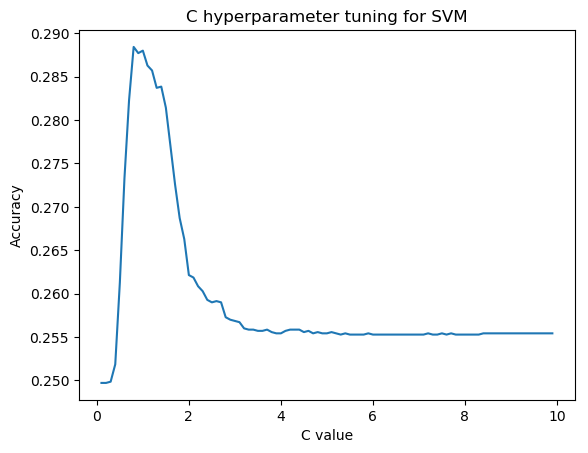
\includegraphics[width=.6\linewidth]{Cross_valid_plots/SVM_C_hyper_fig_fine.png}
  \caption{C fine tuning}
  \label{fig:sub2}
\end{subfigure}
\caption{C hyper parameter tuning}
\label{fig:test}
\end{figure}
 
\newpage
\subsection{K nearest neighbours}
Neighbors-based classification is a type of instance-based learning or non-generalizing learning: it does not attempt to construct a general internal model, but simply stores instances of the training data. Classification is computed from a simple majority vote of the nearest neighbors of each point. Under some circumstances, it is better to weight the neighbours such that nearer neighbours contribute more to the fit i.e. proportional to the inverse of the distance from the query point. As we would like to experiment with both options, we will create two KNN classifiers with two different distance functions and test their performance.
\begin{figure}[h]
\centering
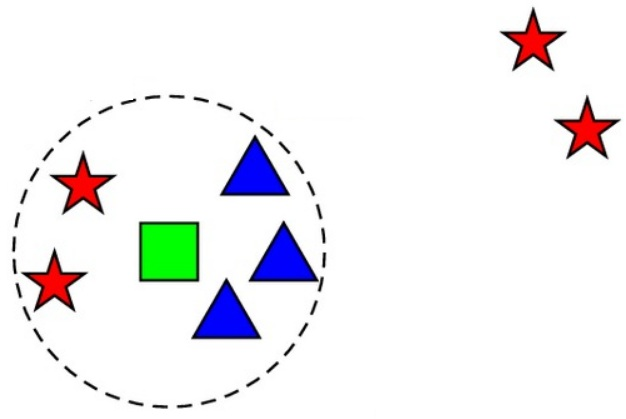
\includegraphics[width=0.3\textwidth]{report_pics/knn}
\caption{Classification depends on weight function}
\end{figure}
To select the right value for k hyper parameter we used the k-fold cross validation technique for both knn models, with different weight types, as shown on below. We ended up with k = 3 after which the accuracy starts to decease. As we clearly can see from the plot, the KNN with distance weights performed better with all values of k.
\begin{figure}[h]
\centering
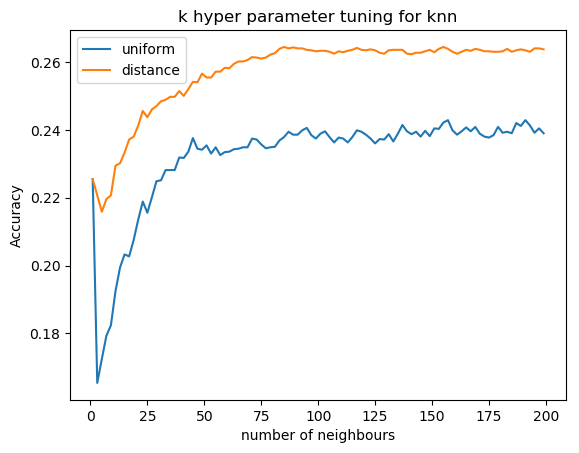
\includegraphics[width=0.6\textwidth]{Cross_valid_plots/k_hyper_fig}
\caption{k hyper parameter tuning}
\end{figure}


\newpage
\subsection{Random Forest}
A random forest is a meta estimator that fits a number of decision tree classifiers on various sub-samples of the dataset and uses averaging to improve the predictive accuracy and control over-fitting. According to \href{https://medium.com/all-things-ai/in-depth-parameter-tuning-for-random-forest-d67bb7e920d}{medium.com post} the most important parameters of this classifier are:
\begin{enumerate}
	\item Number of trees - Usually the higher the number of trees the better to learn the data. However, adding a lot of trees can slow down the training process. Based on the experiments conducted we decided to go with 50 trees as for bigger values we didn't noticed any improvement.
	\item Maximum depth - represents the depth of each tree in the forest. The deeper the tree, the more splits it has and it captures more information about the data. The downside of a deeper tree, that it tends to overfit. Based on the plots we decided to set the depth to 8 as bigger values does not increase accuracy.
	\item Minimum samples split - represents the minimum number of samples required to split an internal node. Large numbers will cause the nodes of the trees not to split at all disabling it's ability to learn. As we can see on the plot, the best accuracy was achieved with the smallest value of 0.01 which means minimum 70 samples for a split.
\end{enumerate}

\begin{figure}[h]
\centering
\begin{subfigure}{0.3\textwidth}
  \centering
  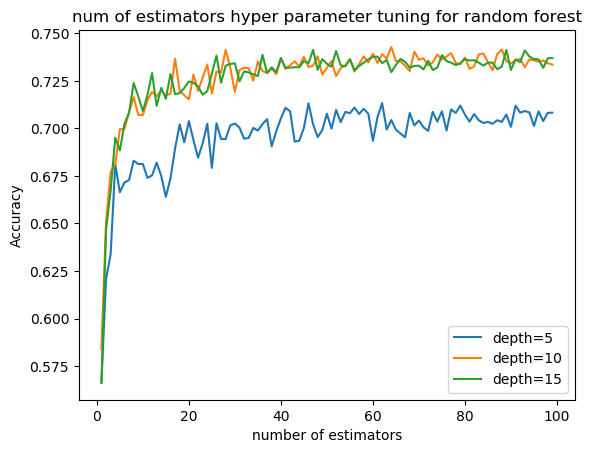
\includegraphics[width=1\linewidth]{Cross_valid_plots/n_hyper_forest_fig}
  \caption{n tuning}
  \label{fig:sub1}
\end{subfigure}%
\begin{subfigure}{0.3\textwidth}
  \centering
  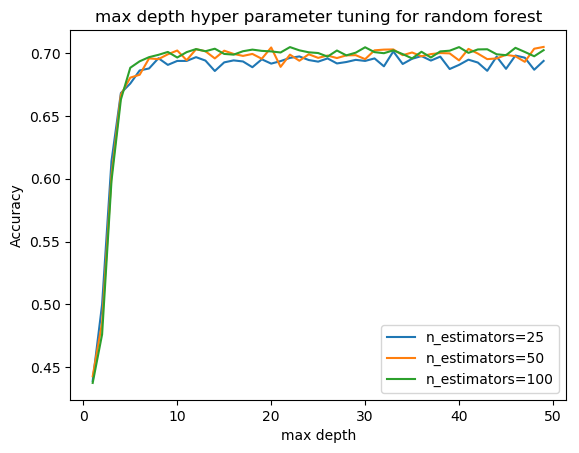
\includegraphics[width=1\linewidth]{Cross_valid_plots/d_hyper_forest_fig}
  \caption{depth tuning}
  \label{fig:sub1}
\end{subfigure}%
\begin{subfigure}{0.3\textwidth}
  \centering
  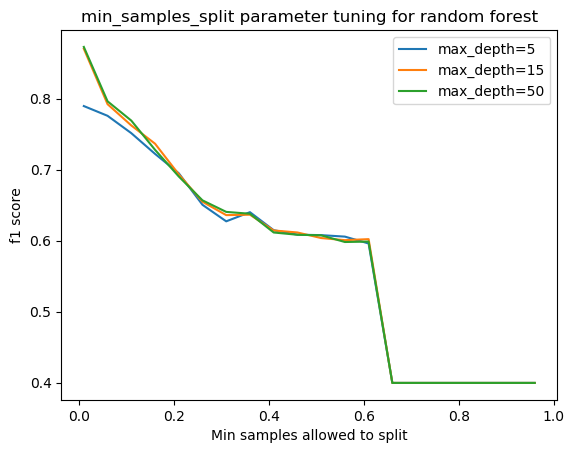
\includegraphics[width=1\linewidth]{Cross_valid_plots/s_hyper_forest_fig}
  \caption{split tuning}
  \label{fig:sub2}
\end{subfigure}
\caption{Random forest parameters tuning}
\label{fig:test}
\end{figure}

We find other parameters less important (and less intuitive), thus we will use the default values.

\newpage
\subsection{Multi-layer perceptron}
Multi-layer Perceptron classifier. This model optimizes the log-loss function using LBFGS or stochastic gradient descent. In this section we discuss the most important parameters of MLP and the values we have chosen. Our decisions mostly based on the post in \href{https://stats.stackexchange.com/questions/181/how-to-choose-the-number-of-hidden-layers-and-nodes-in-a-feedforward-neural-netw}{stats.stackexchange.com}.
\begin{enumerate}
	\item Number of hidden layers - There is a consensus that the situations in which performance improves with a second (or third, etc.) hidden layer are very few. One hidden layer is sufficient for the large majority of problems. Based on this statement we decided to test three options in the cross-validation process: 1, 2 and 3 hidden layers.
	\item Hidden layer size - There is rule of thumb that helps for supervised learning problems. The upper bound on the number of hidden neurons that will not result in over-fitting is:
\begin{gather*}
N_h = \dfrac{N_s}{\alpha * (N_i + N_o)}
\end{gather*}
while $N_o$ is number of output neurons, $N_i$ is number of input neurons, $N_s$ number of training samples and $\alpha$ is arbitrary factor between 2 and 10. In our case, for $\alpha = 10$ 
causing upper bound of 166 neurons in hidden layer. Thus, during cross validation we will test numbers in this range.
	\item Activation function - we decided to use the default option which is ReLU.
\end{enumerate}

We decided to leave other parameters at their default values as the problem of selecting the optimal neural network model is complex by itself and not should be covered in this submission, resulting 2 models trained and tested with different values of hidden layer size. As we can see from the plot, t.  

\begin{figure}[h]
\centering
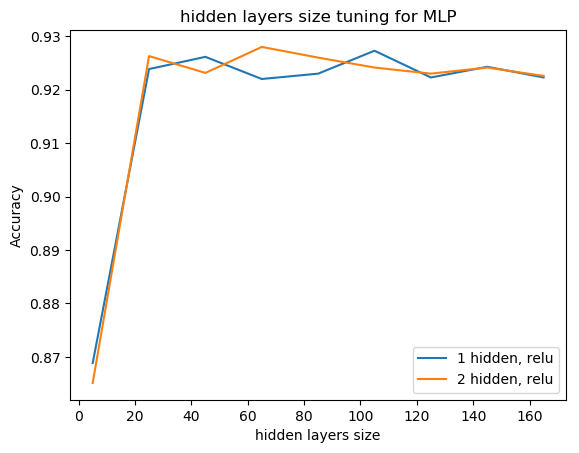
\includegraphics[width=0.5\textwidth]{Cross_valid_plots/mlp_h_fig}
\caption{MLP cross validation results}
\end{figure}

\newpage
\section{Performance measurements}
\subsection{Majority votes measurement}
For the task of prediction which party will win the majority of votes we propose to use the most simple measurement that comes to mind - "binary score": if the majority of predicted tags are from the same class as in validation set, the model score is 1. Unfortunately this method can give us multiple models which can predict the winner party, i.e. it doesn't choose the best model for this task, which means the binary measurement we chose is not good enough as it can't provide us a relative "goodness" of the models which predicted correctly the winner party. To make the method more selective we decided to use f1 score as secondary measurement.

\subsection{Votes division measurement}
For the task of prediction of votes division we want is to predict correctly the division of the total votes (in test set) between the parties, but not a vote of each person. In other words, we want to compare a histogram of predicted votes to the histogram of true votes in the test set, thus the metrics we use is an Euclidean distance between two histograms:
\begin{gather*}
D = \sqrt[2]{\sum_{i=0}^{12} (histPredicted_i - histTrue_i)^2}   
\end{gather*}
According to this measurement, predicted votes distribution histogram which is very different form the true histogram, will be "far away" (in terms of Euclidean distance) from the true votes distribution histogram. On the other hand, predicted votes distribution histogram which is very similar to the true histogram, will be very close to it. Thus, the model with the shortest Euclidean will be considered as the best model for votes division prediction task.

\subsection{Most probable voters measurement}
In this task we should predict a probability of each voter to vote for each party, but not the exact label. That's why the first approach was to use custom metrics for this task.
\begin{figure}[h]
\centering
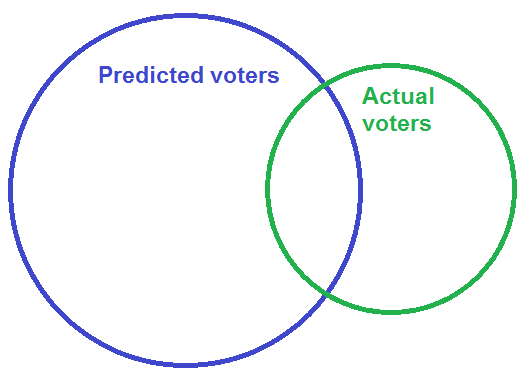
\includegraphics[width=0.3\textwidth]{report_pics/sets}
\caption{Intersection of predicted voters and actual voters of a party}
\end{figure}
Looking at the figure and denoting $P$-as predicted set, $T$-as true set, we can state the following:
\begin{enumerate}
	\item $P \cap T$ - i.e. the set intersection is the actual voters which will be provided with transportation. Generally speaking, big intersection is good, thus it will increase the score.
	\item $P-T$ - are mispredicted voters, which will not vote for the given party, but will get a free ride. Of course that, big $P-T$ is bad, thus it will decrease the score.
	\item $T-P$ - are actual voters which will not get a transportation and maybe will not vote at all as a result. big $T-P$ is bad, thus it will decrease the score.
\end{enumerate} 
Finally we ended up with following score calculation:\\
$P_i \cap T_i$ - actual voters with transportation by party i \\
   $P_i - T_i$ - mispredicted voters, which will not vote party i \\
   $T_i -P_i$ - actual voters of party i, which will not get a transportation \\
\begin{gather*}   
   Score = \sum_{i=0}^{12} |P_i \cap T_i|-|P_i - T_i|-|T_i -P_i|  
\end{gather*}
Interestingly, weighted f1 score perfectly corresponds to our custom score, so it will be used as metrics in this prediction task.  

   

\newpage
\section{Prediction results and chosen model}
In this section we will discuss the results of each prediction task, the quality of the results according to the measurements and which model was selected for each prediction task.
\subsection{Majority votes}
To visualize the prediction results on validation set we will use histogram of true labels of validation set and predicted labels.

\begin{figure}[htp]
\centering
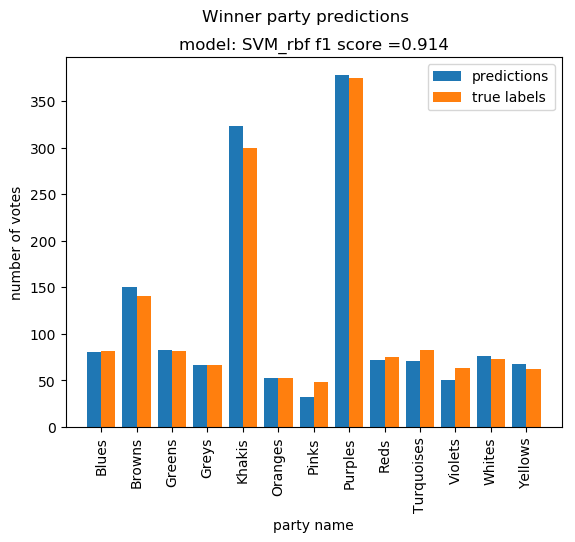
\includegraphics[width=.4\textwidth]{Winner_party_plots/SVM_rbf_fig}
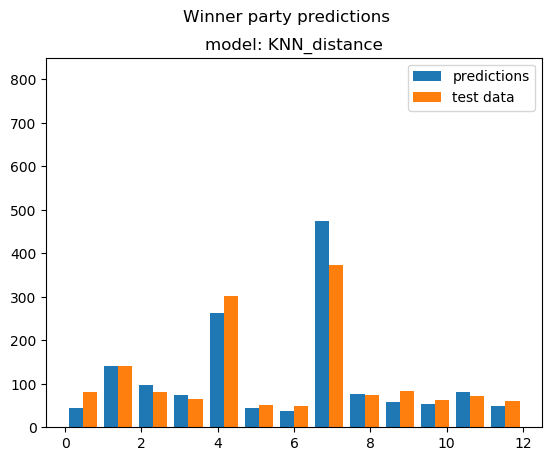
\includegraphics[width=.4\textwidth]{Winner_party_plots/KNN_distance_fig}
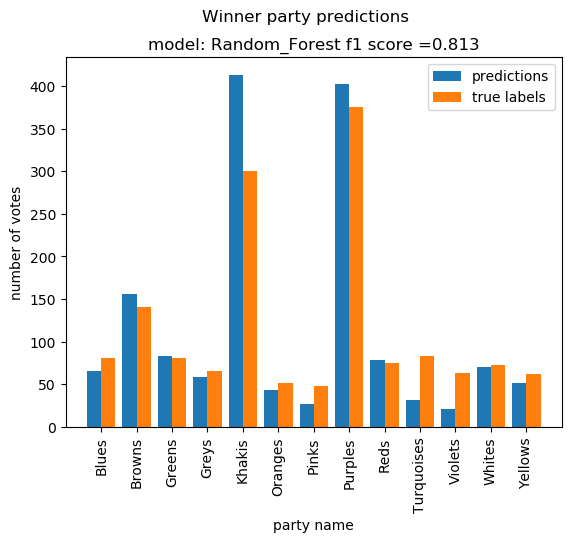
\includegraphics[width=.4\textwidth]{Winner_party_plots/Random_Forest_fig}
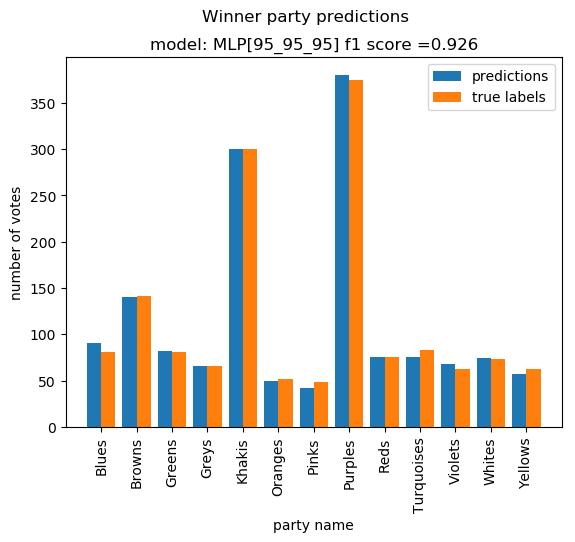
\includegraphics[width=.4\textwidth]{Winner_party_plots/MLP[95_95_95]_fig}
\caption{Votes distribution}
\end{figure}

Looking at the plots we can say that all models predicted the winner correctly, but the MLP model got the highest f1 score, thus it was selected automatically as the best model for this task.

\newpage
\subsection{Votes division}
To visualize the prediction results on validation set we will use histogram of true labels of validation set and predicted labels. According to the metrics we choose for Votes division task, we are interested in model which achieved the smallest Euclidean Distance between the histograms. 

\begin{figure}[htp]
\centering
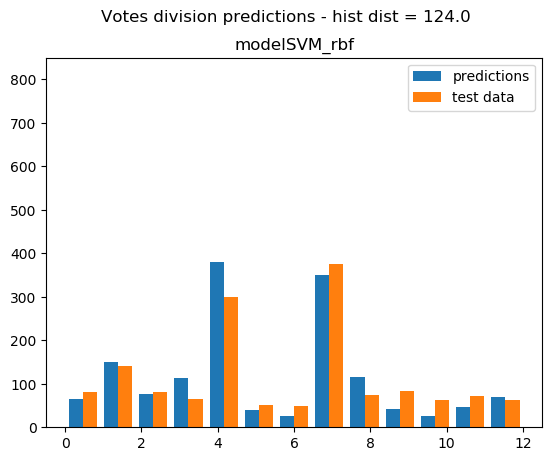
\includegraphics[width=.4\textwidth]{Division_prediction_plots/SVM_rbf_fig}\quad
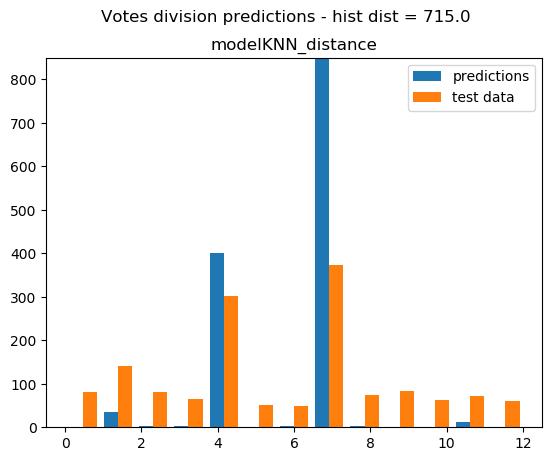
\includegraphics[width=.4\textwidth]{Division_prediction_plots/KNN_distance_fig}\quad
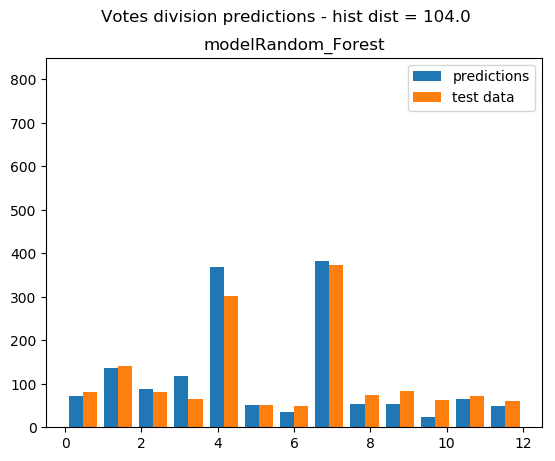
\includegraphics[width=.4\textwidth]{Division_prediction_plots/Random_Forest_fig}
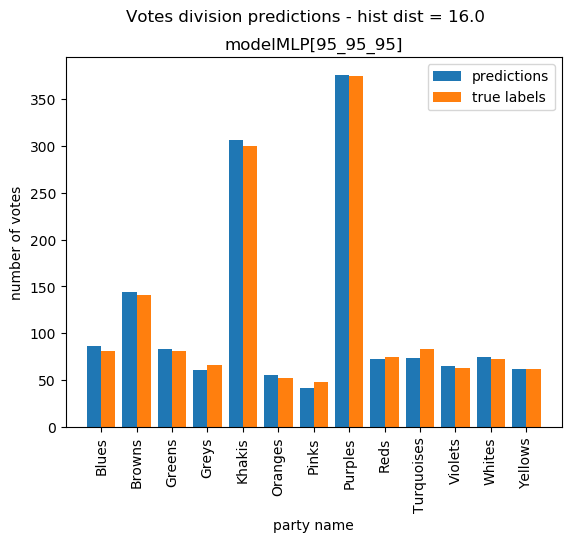
\includegraphics[width=.4\textwidth]{Division_prediction_plots/MLP[95_95_95]_fig}
\caption{Votes distribution}
\end{figure}

Looking at the plot we can clearly see that model performance corresponds to the chosen metrics, i.e. the euclidean norm. As stated in previous sections, the most similar histograms have the smallest euclidean distance. In conclusion, MLP classifier achieved best performance on validation set with final score of 18, which is the best score among other classifiers. 

\newpage
\subsection{Voters transportation}
To visualize the prediction results on validation set we will use bar chart. Each color represents a set of one type, and the bar height, the size of the set. The grey color is a sets of "forgotten" voters, i.e. the voters who are willing to vote for a given party, but not been provided by a transportation. The red color is a sets of votes who are not voting for the party but still got a free ride. The green bar is the voters which will vote and actually get a transportation. Grey and the red bars height effects negatively on the score, while green bar effects positively.    
\begin{figure}[h]
\centering
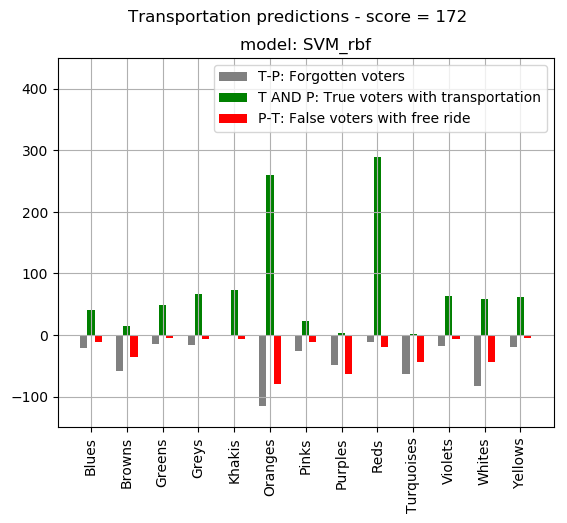
\includegraphics[width=.4\linewidth]{Vote_prediction_plots/SVM_rbf_fig.png}
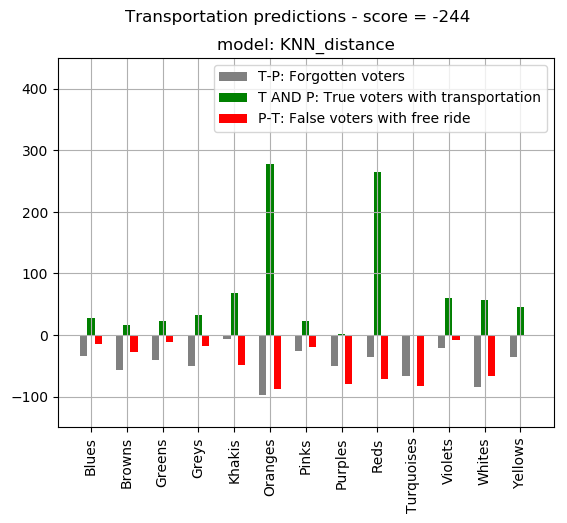
\includegraphics[width=.4\linewidth]{Vote_prediction_plots/KNN_distance_fig}
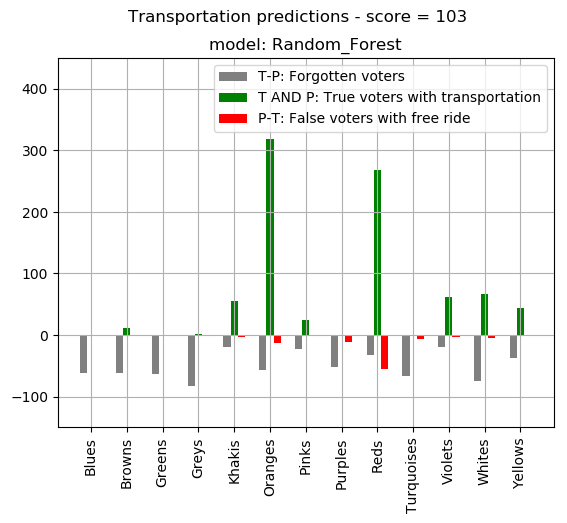
\includegraphics[width=.4\linewidth]{Vote_prediction_plots/Random_Forest_fig}
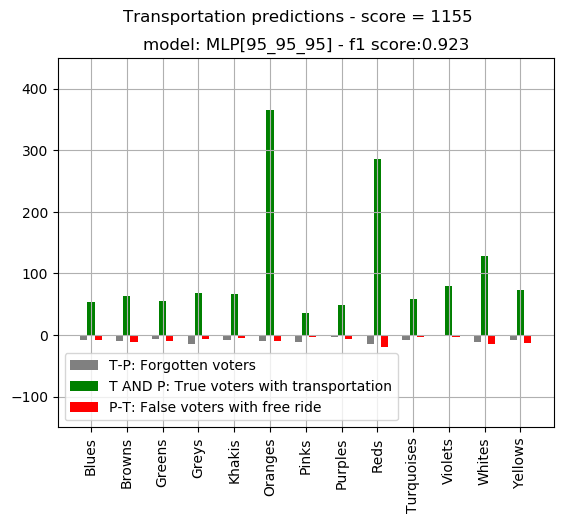
\includegraphics[width=.4\linewidth]{Vote_prediction_plots/MLP[95_95_95]_fig}
\caption{Models performance for transportation task}
\label{fig:test}
\end{figure}

As we can see on the plots, Random Forest has very low performance score, which means according to it's probability predictions the parties will not provide transportation to their potential voters or will give a free ride to people who doesn't want to vote for them. On the other hand, MLP was much more accurate with it's probability predictions and provided each party a relatively large list of true potential voters. It's important to mention that the probability threshold we used to visualization is $0.5$, i.e. the person added to the party's list only if he will vote to this party with probability higher than $0.5$. Our implementation provides the functionality the set the probability threshold which will maybe change the list of predicted votes, but not change the model, as it's been selected according to f1 score. 


\newpage
\section{Final answers}
In this section we provide the final answers for the first two prediction tasks and a confusion matrix of the vote prediction of each voter in a test set. First of all the best models are:

\begin{verbatim}
best model for transportation is  MLP[95_95_95]
best model for winner prediction is  MLP[95_95_95]
best model for vote division is  MLP[95_95_95]
\end{verbatim}

\subsection{Which party will win}
As described previously, the best model for this task is SVM with RBF kernel, and its final prediction was:
\begin{verbatim}
MLP[95_95_95]  prediction -  Purples  party will win the elections.
\end{verbatim}

\subsection{Votes division}
As described previously, the best model for this task is Random Forest, and its final prediction was:
\begin{verbatim}
MLP[95_95_95]  prediction - Vote division:
Party  Blues : 5.6 %
Party  Browns : 9.0 %
Party  Greens : 5.5 %
Party  Greys : 4.5 %
Party  Khakis : 21.0 %
Party  Oranges : 2.9 %
Party  Pinks : 3.2 %
Party  Purples : 25.0 %
Party  Reds : 5.1 %
Party  Turquoises : 5.3 %
Party  Violets : 3.3 %
Party  Whites : 5.2 %
Party  Yellows : 4.3 %
\end{verbatim}

\newpage
\subsection{Confusion matrix and test error}
\begin{figure}[htp]
\centering
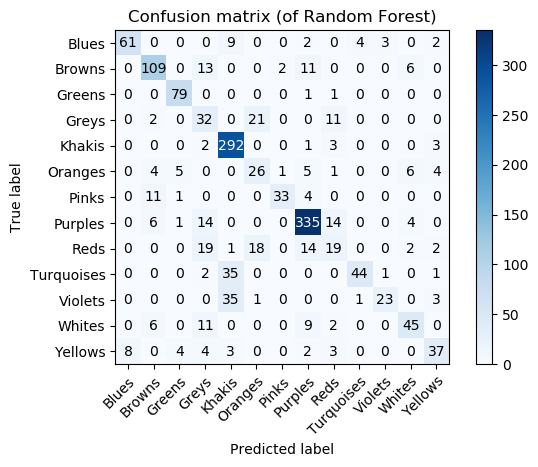
\includegraphics[width=\textwidth]{confusion_matrix/confusion_fig}
\caption{Confusion matrix of MLP}
\end{figure}

\begin{verbatim}
Model  MLP[95_95_95]  reached  6.4 % error.
\end{verbatim}

\newpage
\section{Comparison with one model approach}
In addition to "different model for each task" selection we want to try the "one mode" approach. In this section we will answer the same questions as in our prediction tasks, add a confusion matrix and test error result.
\subsection{How do we select the best model}
We decided to create automatic model selection process in the same class $modelSelector$ which selects one model for all tasks by executing a two stage process:
\begin{enumerate}
\item Evaluate all candidate models on validation set and select all the models which predicted correctly the winner party. We see this task as the most important as it predicts who is the winner - the most important outcome of the elections.
\item Evaluate all selected models on validation set to predict the most probable voters for the transportation task, and select the model which performed better than others according to metrics of this task. We see the transportation task as the second important task as a serious financial investment involved in it. Finally, the model with best performance selected as "one for all" model. 
\end{enumerate}
It's worth to mention that we don't evaluate the model on the validation set to get a score for the votes division task, as wee see this task least important. Moreover, as we can see from our previous results, a model with best transportation task score, actually handles very good the vote division task as well. Finally, the best for all model was MLP. As we saw in previous section, this model was selected for each prediction task independently, so the final results are exactly the same.  

\subsection{Comparison}
As we can see, in both cases we achieved same results as the same model was selected. The main advantage of one for all method is simplicity of implementation.

\newpage
\section{Feature manipulation}
In this section we will describe our implementation of bonus part of feature manipulation which will cause other party to win. To complete this task we've created a class $featureManipulator$ which automatically finds features which will cause other party to win. Firstly, we provides the class the best model for winner party prediction. Them, in iterative manner, Feature Manipulator decreases or increases one column of the validation or test data one by one, by a given constant $C$. In each iteration we start with relatively small values of $C$ and increase them gradually, until the model predicts another party as a winner. To visualize it we plot an histogram of original predictions, new predictions on altered data and true labels.   

\begin{figure}[ht]
	\centering
	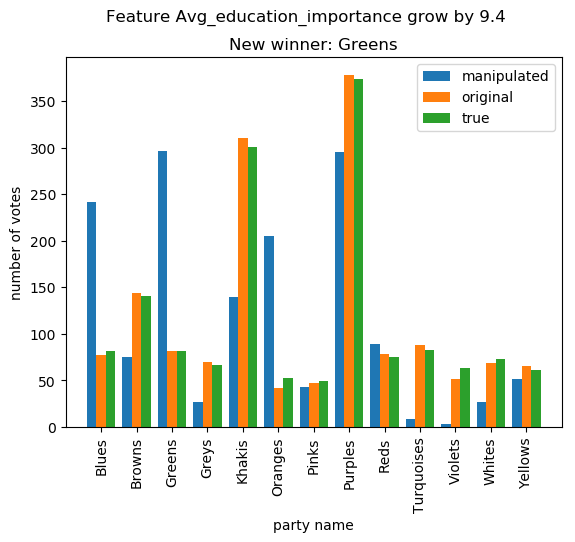
\includegraphics[width=0.2\textwidth]{dramatic_feature/Avg_education_importance_increased}
	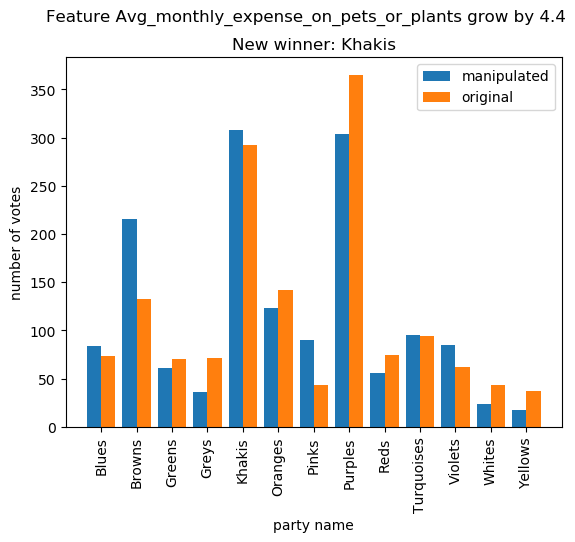
\includegraphics[width=0.2\textwidth]{dramatic_feature/Avg_monthly_expense_on_pets_or_plants_increased}
	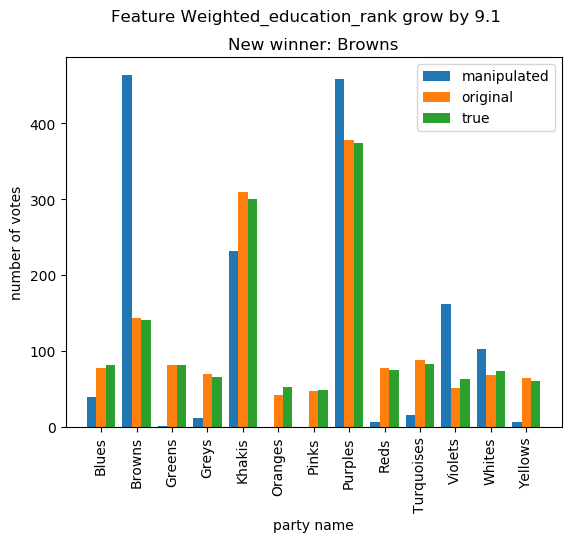
\includegraphics[width=0.2\textwidth]{dramatic_feature/Weighted_education_rank_increased}	
	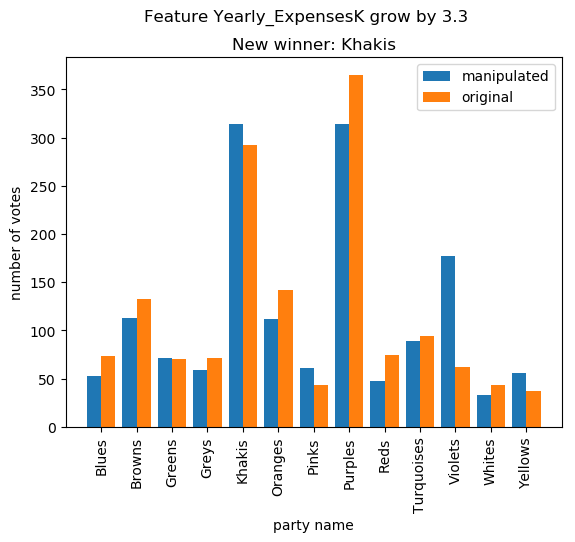
\includegraphics[width=0.2\textwidth]{dramatic_feature/Yearly_ExpensesK_increased}					
\end{figure}

To summarize the results:

\begin{enumerate}

\item If Weighted education rank  will grow by  9.1 , that will cause  Browns  to win

\item If  Avg environmental importance  will grow by  5.8 , that will cause  Blues  to win

\item If  Avg education importance  will grow by  9.4 , that will cause  Greens  to win

\item If  Avg monthly expense on pets or plants will grow by  11.3 , that will cause  Yellows  to win

\item If  Yearly Expenses K  will grow by  2.9 , that will cause  Khakis  to win

\end{enumerate}

\newpage
\section{D}
\subsection{C}
\subsection{A}
\subsection{B}
\subsection{C}

\begin{enumerate}
	\item one
	\item two
\end{enumerate}

\end{document}
